\documentclass{beamer}
\usepackage{graphicx}
\usepackage{paralist}
\usepackage{outlines}

\title{History Panel and Brushes}
\author{Mendocino College - Digital Image Manipulation with Photoshop}
\titlegraphic{\vspace{-10mm}
\includegraphics[width = .9\textwidth]{images/photoshop.jpg}} 
\date{\vspace{-5em}} 


\mode <presentation>
\usetheme{Warsaw}
\usecolortheme{default}

\setbeamerfont{footline}{size=\fontsize{5}{8}\selectfont}

\definecolor{darkred}{rgb}{20,0,0}
\definecolor{darkgreen}{RGB}{40,110,20}
\definecolor{darkpurple}{RGB}{30,0,30}
\definecolor{chardonnay}{RGB}{255, 255, 204}

\setbeamercolor*{palette primary}{fg=white, bg=darkgreen}


\begin{document}
	{
		\setbeamertemplate{footline}{} 
		\setbeamertemplate{headline}{} 
		\begin{frame}
			\vspace{-35pt}
			\maketitle
		\end{frame}
	}
		
		
\section{History Panel}

\subsection{History Panel}		

	\begin{frame}
		\frametitle{History Panel}
		\begin{outline}
			\1 Use the Undo/Redo commands and the History panel to control the state of your images in Adobe Photoshop.
			\1 Each time you apply a change to an image, the new state of that image is added to the panel.
			\1 You can use the History panel to jump to any recent state of the image created during the current working session.
			\1 For example:  When you select, paint, and rotate part of an image, each of those states is listed separately in the panel.
			\2 When you select one of the states, the image reverts to how it looked when that change was first applied. 
			\2 You can then work from that state.
			\1 You can also use the History panel to delete image states and, in Photoshop, to create a document from a state or snapshot.
			\1 You can use the History panel to create a document from a state or snapshot.
		\end{outline}
	\end{frame}

	\begin{frame}
	\frametitle{How to use the History Panel}
	\begin{outline}
		\1 To display the History panel: 
		\2 Click Window in the menu bar on top, 
		\2 then select History. 
		\1 Click the name of the state in the history panel to revert to that image state.
		\2 This will cause the states below it to become grey.
		\2 The previous states will remain available to go back and forth from,
		\2 but once you make a new change, it will delete all history states below it, in place of the new change.
		\1 Delete states by dragging them to the delete icon (
\includegraphics[width=0.05\textwidth]{images/history panel - trash bin.PNG}).
		\2 This is irreversible.    
		\1 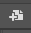
\includegraphics[width=0.05\textwidth]{images/history panel - create new document from current state.png} Creates a new document (image) from the currently selected state.
	\end{outline}
\end{frame}

	\begin{frame}
	\frametitle{History Panel Snapshots}
	\begin{outline}
		\1 Snapshots let you make a temporary copy (or snapshot) of any state of the image. 
		\1 The new snapshot is added to the list of snapshots at the top of the History panel. They allow you to easily recover your work, and allow you to easily revert back to specific states while experimenting with complex techniques.  
		\1 Selecting a snapshot lets you work from that version of the image.
		\1 Snapshots can be stored for an entire work session, but are not saved with an image and will be deleted when the image is closed.
		\1 To select a snapshot, click the name of the snapshot.		
		\1 Rename a snapshot by double-clicking it and enter a name.
		\1 To delete a snapshot, select the snapshot and either choose Delete from the panel menu, then click the Delete icon.
	\end{outline}
\end{frame}

\subsection{Example}		
	\begin{frame}
		\frametitle{History Panel Example}
		\begin{center}
			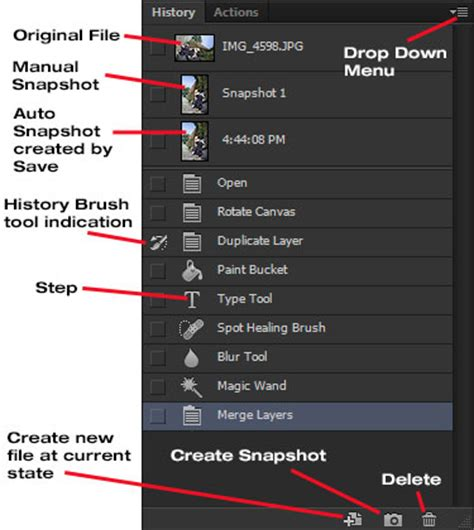
\includegraphics[width=0.6\textwidth]{images/history panel.png}
		\end{center}
	\end{frame}

\subsection{Options}		
	\begin{frame}
		\frametitle{History Panel Options}
		\begin{outline}
			\1 The History panel lists the previous 20 states, by default. 
			\2 You can change the number of remembered states by setting a preference under Preferences $\rightarrow$ Performance. 
			\2 Older states are automatically deleted to free more memory for Photoshop. 
			\2 To keep a particular state throughout your work session, make a snapshot of the state.
		\end{outline}
	\end{frame}

\subsection{Resources}		
	\begin{frame}
		\frametitle{Additional Resources for the History Panel}
		\begin{outline}
			\1 Undo/redo and history in Adobe Photoshop
			\2 By:  Adobe
			\2 https://helpx.adobe.com/photoshop/using/undo-history.html
		\end{outline}
	\end{frame}


\section{History Brush}

\subsection{History Brush}		

\begin{frame}
	\frametitle{History Brush}
	\begin{outline}
		\1 The History Brush tool allows you to restore parts of an image to an earlier history state by painting over them.
		\1 This tool makes a copy (sample) of the image, and then paints with it.
		\1 The History Brush tool copies from one state or snapshot to another, but only at the same location.
		\1 For example:  
		\2 You make a snapshot of a change you made with a painting tool or filter (with the Full Document option selected when you create the snapshot). 
		\2 After undoing the change to the image, you use the History Brush tool to apply the change selectively to areas of the image. 
		\2 The History Brush tool paints from a layer in the selected state to the same layer in another state, unless you select a merged snapshot, 
	\end{outline}
\end{frame}

\begin{frame}
	\frametitle{How to Use the History Brush Tool}
	\begin{outline}
		\1 Choose Window $\rightarrow$ History to open the History panel.  
		\1 In the History panel, click the far-left column of the state that you want to use as the source for the History Brush tool. 
		\2 A brush icon will appear next to the selected history state.
		\1 Select the History Brush tool (Y) 
\includegraphics[width=0.04\textwidth]{images/P_HistoryBrush_Lg_N.png}
		\1 Use the Options bar to customize tool settings, like Size and Hardness, to get the effect you want.
		\1 Drag over the parts of the image you want to restore.
	\end{outline}
\end{frame}

\subsection{Example}		
\begin{frame}
	\frametitle{History Brush Example}
	\begin{center}
		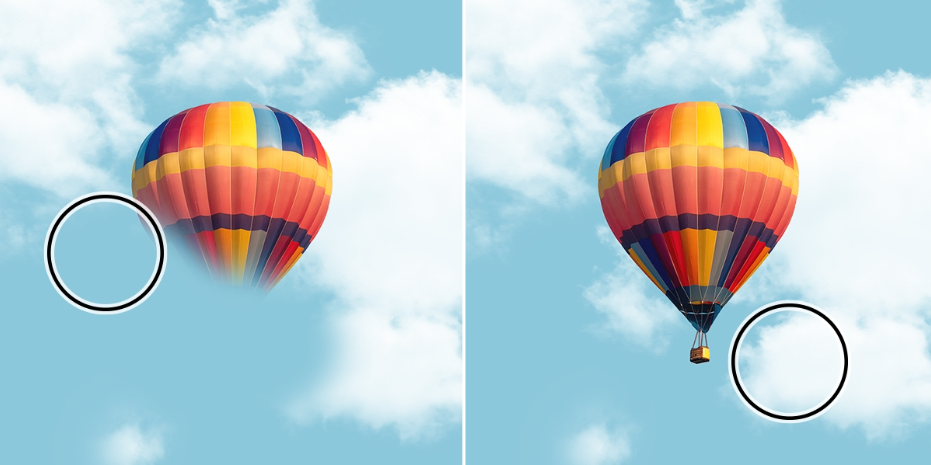
\includegraphics[width=1.0\textwidth]{images/history brush tool.png}
	\end{center}
\end{frame}

\subsection{Options}		
\begin{frame}
	\frametitle{History Brush Options}
	\begin{outline}
		\1 Opacity and Flow
		\1 Blending Modes
		\1 Brushes and Size/Hardness
	\end{outline}
\end{frame}

\subsection{Resources}		
\begin{frame}
	\frametitle{Additional Resources for the History Brush}
	\begin{outline}
			\1 Restore parts of an image with the History Brush tool
			\2 By:  Adobe
			\2 https://helpx.adobe.com/photoshop/using/tool-techniques/history-brush-tool.html
			\1 Anyone can create incredible paintings in Photoshop with a single tool!
			\2 Texturelabs
			\2 https://www.youtube.com/watch?v=U7SnfuIM778
	\end{outline}
\end{frame}


\section{Art History Brush}

\subsection{Art History Brush Tool}		

\begin{frame}
	\frametitle{Art History Brush}
	\begin{outline}
		\1 The Art History Brush tool paints with stylized strokes, using the source data from a specified history state or snapshot.
		\1 You can also paint with the Art History Brush tool to create special effects.
		\1 The Art History Brush tool uses a specified history state or snapshot as the source data, and uses that data along with the options you set to create different colors and artistic styles.
		\1 By working with different paint style, size, and tolerance options, you can simulate the texture of painting with different colors and artistic styles.
		\1 For various visual effects, experiment with applying filters or filling an image with a solid color before painting with the Art History Brush tool. 
	\end{outline}
\end{frame}

\begin{frame}
	\frametitle{How to Use the Art History Brush Tool}
	\begin{outline}
		\1 In the History panel, click the left column of the state or snapshot to use as the source for the Art History Brush tool. 
		\2 A brush icon appears next to the source history state.
		\1 Select the History Brush tool (Y) 
\includegraphics[width=0.04\textwidth]{images/P_HistoryArtBrush_Lg_N.png}
		\1 Set Options
		\1 Drag over the parts of the image you want to restore.
	\end{outline}
\end{frame}

\subsection{Example}		
\begin{frame}
	\frametitle{Art History Brush Example}
	\begin{center}
		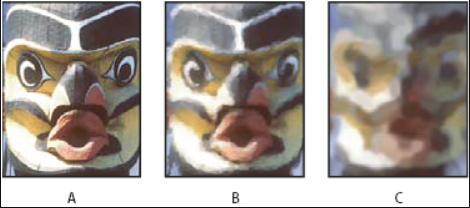
\includegraphics[width=1.0\textwidth]{images/art history brush example.png}
	\end{center}
\end{frame}

\subsection{Options}		
\begin{frame}
	\frametitle{Art History Brush Options}
	\begin{outline}
		\1 Choose a brush from the Brush Presets picker, and set brush options.
		\1 Choose a blending mode from the Mode menu. 
		\1 Choose an option from the Style menu to control the shape of the paint stroke.
		\1 For Area, enter a value to specify the area covered by the paint strokes. 
		\2 The greater the size, the larger the covered area and the more numerous the strokes.
		\1 For Tolerance, enter a value to limit the regions where paint strokes can be applied. 
		\2 A low tolerance lets you paint unlimited strokes anywhere in the image. 
		\2 A high tolerance limits paint strokes to areas that differ considerably from the color in the source state or snapshot.
	\end{outline}
\end{frame}

\subsection{Resources}		
\begin{frame}
	\frametitle{Additional Resources for the Art History Brush}
	\begin{outline}
		\1 Paint with the Art History Brush in Photoshop
		\2 By:  Adobe
		\2 https://helpx.adobe.com/photoshop/using/painting-stylized-strokes-art-history.html
		\1 Painted Effect with the Art History Brush - Photoshop Tutorial
		\2 By:  tutvid
		\2 https://www.youtube.com/watch?v=7jjiHwKQGkc
	\end{outline}
\end{frame}
	
\end{document}